% Doi ten hinh sang figures/multitask_architecture.png (hoac copy file) truoc khi \input.
% Style dong bo voi rivf_paper/chapters/figure/fig1_architecture.tex.
\begin{figure*}[!t]
    \centering
    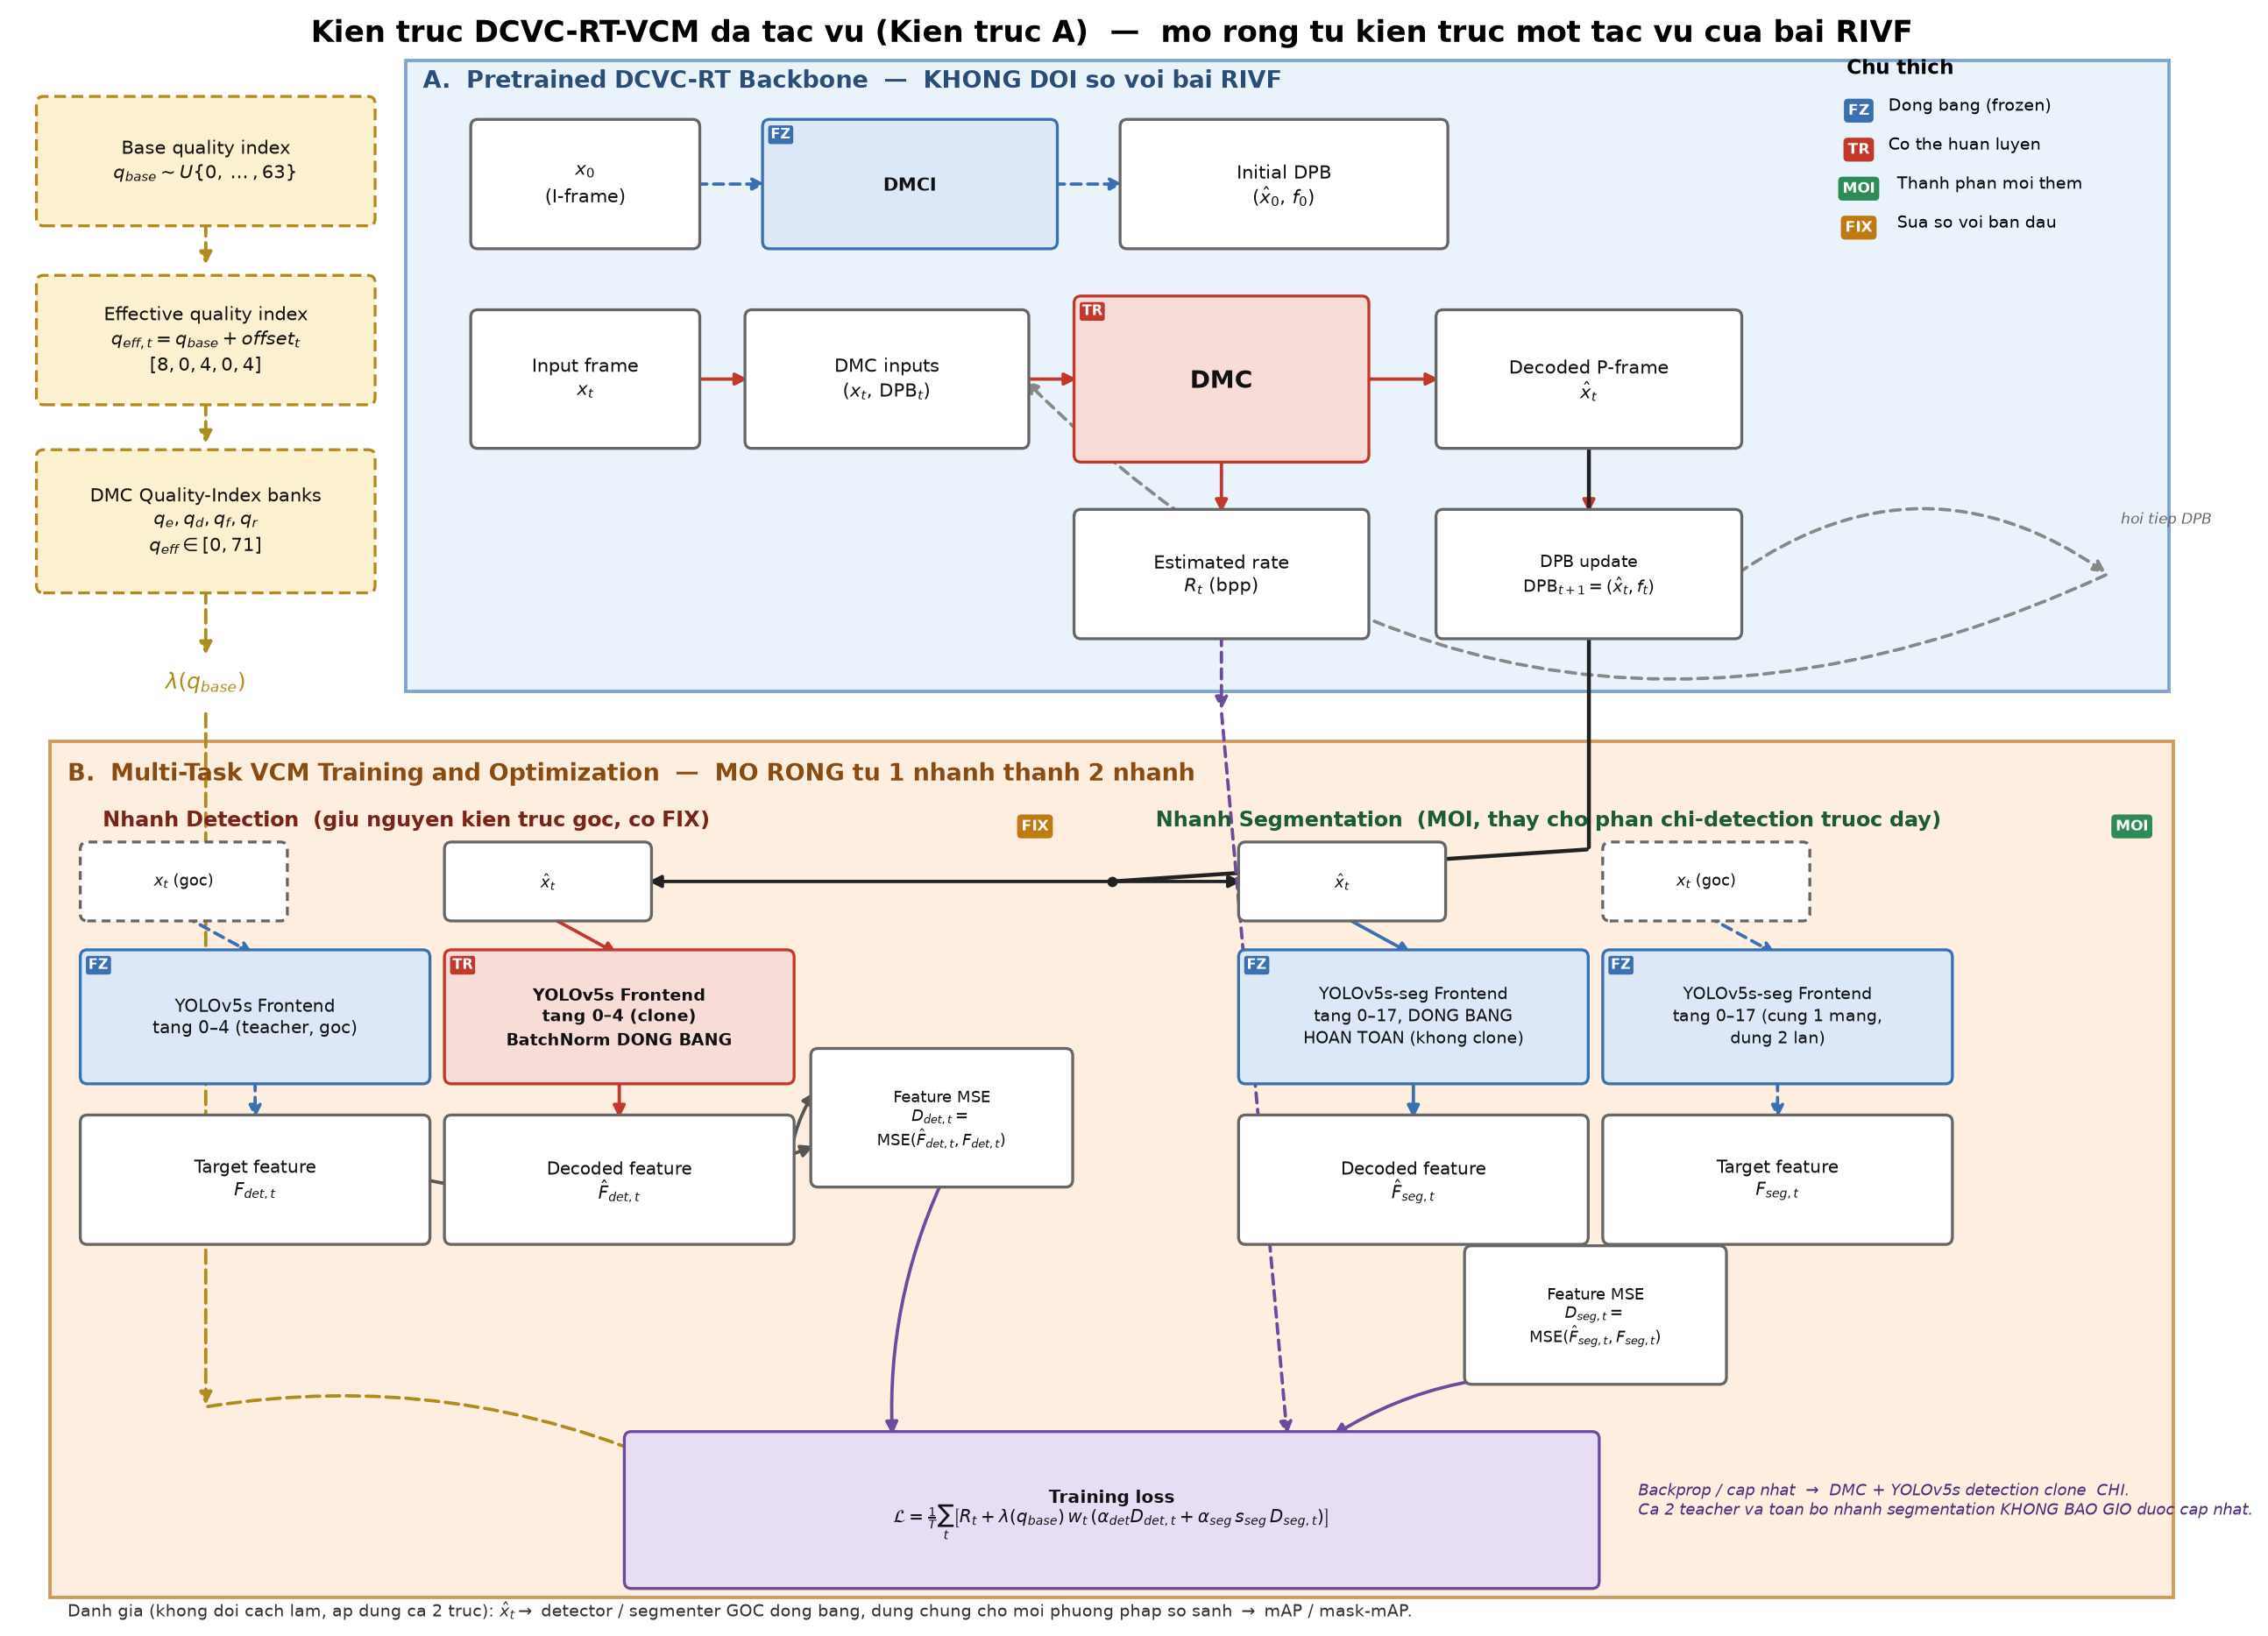
\includegraphics[width=\textwidth]{multitask_architecture.png}
    \caption{Overall architecture of the multi-task extension, built on
    top of \method{}'s single-task architecture (Fig.~2). Region A (the
    DCVC-RT backbone) is unchanged. Region B extends from a single
    detection branch into two parallel branches: detection keeps the
    original architecture but freezes the cloned front end's BatchNorm
    in eval mode throughout training (\textsc{fix}), and segmentation
    is an entirely new, fully frozen branch supervised at layer 17
    (\textsc{new}). Evaluation still uses separate, pretrained
    detector/segmenter models shared by every compared method.}
    \label{fig:multitask-architecture}
\end{figure*}
